\begin{figure*}[!h]
  \centering
  \begin{subfigure}[t]{0.3\textwidth}
	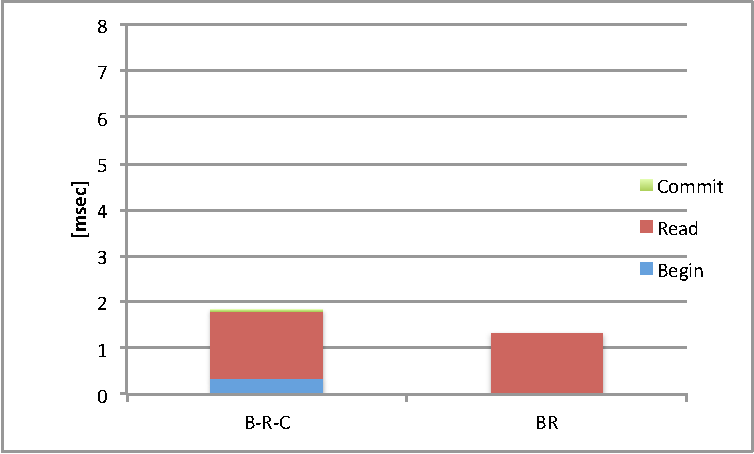
\includegraphics[width=\textwidth]{figs/read_latency.pdf}
	\caption[]{Read}
    \label{fig:latency:read}
  \end{subfigure}
  \begin{subfigure}[t]{0.3\textwidth}
	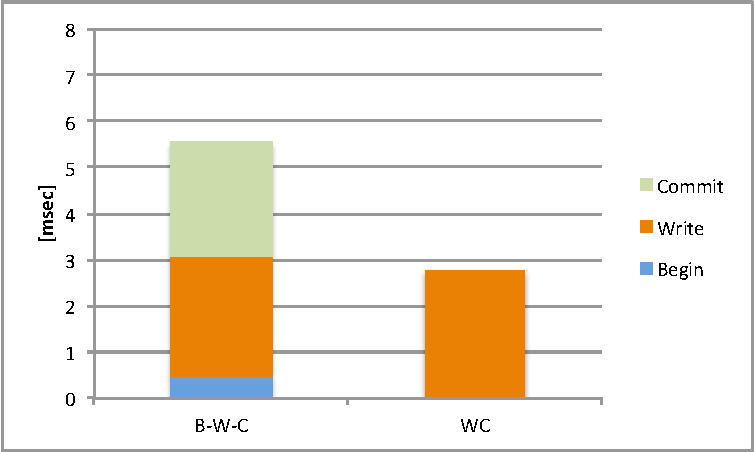
\includegraphics[width=\textwidth]{figs/write_latency.pdf}
	\caption[]{Write}
        \label{fig:latency:write}
  \end{subfigure}	
  \begin{subfigure}[t]{0.3\textwidth}
	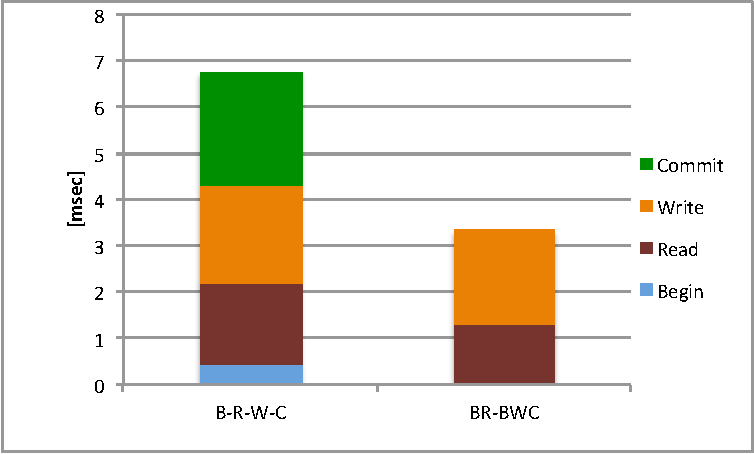
\includegraphics[width=\textwidth]{figs/rmw_latency.pdf}
	\caption[]{Read Modify Write}
    \label{fig:latency:rmw}
  \end{subfigure}			
  \caption{Breakdown of transaction latency}
  \label{fig:latency}
\end{figure*}


\begin{figure}[!h]
  \centering
  \begin{subfigure}[t]{0.4\textwidth}
	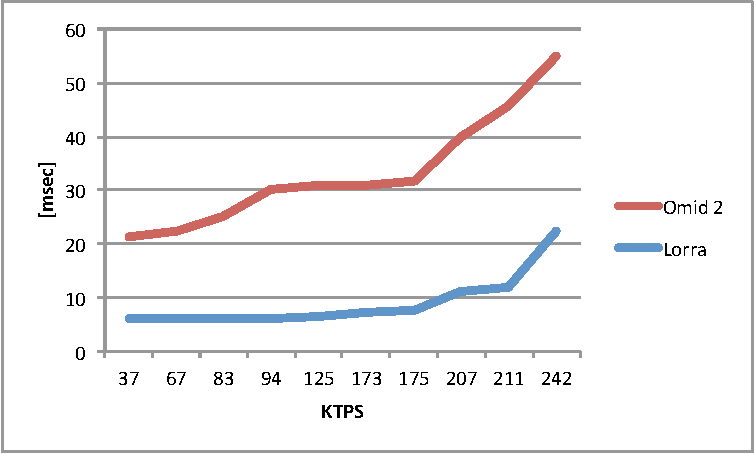
\includegraphics[width=\textwidth]{figs/LL_tx1.pdf}
	\caption[]{Transaction of size 1 latency}
    \label{fig:ll:tx1}
  \end{subfigure}
  \begin{subfigure}[t]{0.4\textwidth}
	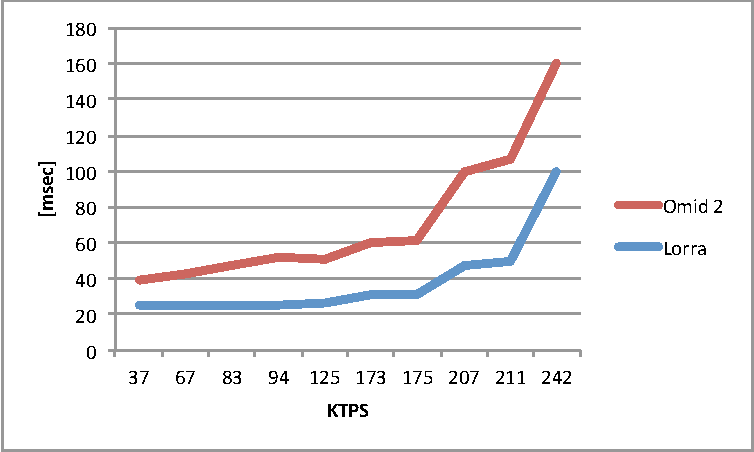
\includegraphics[width=\textwidth]{figs/LL_tx5.pdf}
	\caption[]{Transaction of size 5 latency}
    \label{fig:l:tx5}
  \end{subfigure}			
  \caption{A Comparison between Omid 2 centralized txn entry and \sys's distributed txn entry.}
  \label{fig:ll}
\end{figure}



This section reports the evaluation results of \sys.

\paragraph{Methodology}
To evaluate \sys, we set up a 3 node Hbase cluster loaded with 50GB of data, and a machine hosting the TSO.
Another machine created load on the system by running threads that generated random transactions towards Hbase and the TSO. Transaction size had a zipfian distribution from 1 to 10.
To measure the latency of transactions we modified YCSB~\cite{Cooper:2010:BCS:1807128.1807152} to perform a begin and commit towards the TSO at the beginning and end of each transaction, and used YCSB framework to measure the latency of each stage.

\paragraph{FP API latency}
Figure~\ref{fig:latency} compares the latency observed by YCSB when running regular and FP transactions.
We focus on 3 types of transactions: (1) Read, (2) Write and (3) Read modify write.

Figures~\ref{fig:latency:read} and \ref{fig:latency:write} show the latency of a single read and write transaction. Regular transactions (b-r-c, b-w-c) query the TSO at the begin and commit stage which add 0.3ms for read transactions and 3ms for write transactions.
Figure~\ref{fig:latency:rmw} compares the latency of a read modify write transaction, once using the FP API (br-bwc) and once using the regular transaction API (b-r-w-c).The begin and commit stage of the regular transaction add 3ms to each transaction.

\paragraph{Distributed txn entry}
We now compare \sys's distributed txn entry approach to Omid 2 centralized approach. Figure~\ref{fig:ll} shows the latency of a transaction while applying increasing load on the system. The load is measured in kilo transactions per second (KTPS), and the transaction latency is measured in milliseconds. Figure~\ref{fig:ll:tx1} shows the latency of a transaction with a single read or write. The figure shows that latency obtained by \sys\ is \speedup{4} faster than Omid 2. \sys\ performs better because Omid 2 is throughput oriented and batches the writes to txn entries, so on every begin stage the client has to wait for all commits in the batch to get persistent.
Figure~\ref{fig:ll:tx1} shows the latency of transactions with 5 read or write operations. This time the latency obtained by \sys\ is \speedup{1.8} faster than Omid 2. For transactions with 5 operations to an Hbase table, the begin and commit time become negligible.





\Yoni{
  --background noise
  --switch order of charts
  --explain that the LL is better for all TPS so it doesnt matter the point we choose to check}
